% Created 2023-01-13 Παρ 18:12
% Intended LaTeX compiler: pdflatex
\documentclass[11pt]{article}
\usepackage[utf8]{inputenc}
\usepackage[T1]{fontenc}
\usepackage{graphicx}
\usepackage{longtable}
\usepackage{wrapfig}
\usepackage{rotating}
\usepackage[normalem]{ulem}
\usepackage{amsmath}
\usepackage{amssymb}
\usepackage{capt-of}
\usepackage{hyperref}
\usepackage{booktabs}
\usepackage{import}
\usepackage[LGR, T1]{fontenc}
\usepackage[greek, english]{babel}
\usepackage{alphabeta}
\usepackage{esint}
\usepackage{mathtools}
\usepackage{esdiff}
\usepackage{makeidx}
\usepackage{glossaries}
\usepackage{newfloat}
\usepackage{minted}
\usepackage{chemfig}
\usepackage{svg}
\usepackage[a4paper, margin=3cm]{geometry}
\author{Θεωφανώ Αντωνία Πόταρη, Στυλιανή Σταύρου}
\date{\today}
\title{Ανάλυση των blocks 600-700 - Παραγωγή και Καθαρισμός της Κυκλοπεντανόνης}
\hypersetup{
 pdfauthor={Θεωφανώ Αντωνία Πόταρη, Στυλιανή Σταύρου},
 pdftitle={Ανάλυση των blocks 600-700 - Παραγωγή και Καθαρισμός της Κυκλοπεντανόνης},
 pdfkeywords={},
 pdfsubject={},
 pdfcreator={Emacs 28.2 (Org mode 9.5.5)}, 
 pdflang={English}}
\makeatletter
\newcommand{\citeprocitem}[2]{\hyper@linkstart{cite}{citeproc_bib_item_#1}#2\hyper@linkend}
\makeatother

\usepackage[notquote]{hanging}
\begin{document}

\maketitle
\tableofcontents

\renewcommand{\abstractname}{Περίληψη}
\renewcommand{\tablename}{Πίνακας}
\renewcommand{\figurename}{Σχήμα}
\renewcommand\listingscaption{Κώδικας}

\section{Block 600 - Παραγωγή Κυκλοπεντανόνης με την Φουρφουράλη ως ενδιάμεσο προϊόν}
\label{sec:org96b5c84}

\subsection{Διάγραμμα ροής και Επεξήγηση}
\label{sec:orgb959a8f}
\begin{figure}[htbp]
\centering
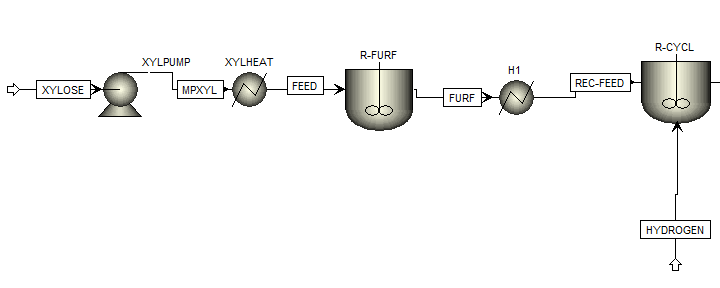
\includegraphics[width=.9\linewidth]{Block_600_-_Παραγωγή_Κυκλοπεντανόνης_με_την_Φουρφουράλη_ως_ενδιάμεσο_προϊόν/2023-01-13_17-51-52_screenshot.png}
\caption{Διάγραμμα ροής του block 600}
\end{figure}

Η κυκλοπεντανόνη παράγεται από τη προσθήκη υδρογόνου στο ενδιάμεσο
προϊόν της διαδικασίας που ονομάζεται φουρφουράλη, η οποία προέρχεται
από την αφυδάτωση στης ξυλόζης. Για αυτό το στάδιο, λοιπόν, από το steam
explosion αξιοποιείται το ρεύμα της ημικυτταρινικής φάσης της βιομάζας
που περιέχει ως κύριο συστατικό την ξυλόζη και εισέρχεται στο block
διεργασίας 600. Στη παρούσα εργασία έχει γίνει η παραδοχή ότι η
ημικυτταρινική φάση αποτελείται από καθαρό ρεύμα ξυλόζης, βέβαια στην
πραγματικότητα το ρεύμα έχει και άλλα συστατικά τα οποία πρέπει να
ληφθούν υπόψιν. Οι εναλλάκτες και η αντλία της διάταξης είναι για να λειτουργεί το σύστημα στις σωστές συνθήκες πίεσης και θερμοκρασίας κάθε αντιδραστήρα.

\subsection{Παραγωγή φουρφουράλης}
\label{sec:org7b0e428}
\subsubsection{Σχεδιαστικές Επιλογές}
\label{sec:orgaef1523}
Για το block 600 οι δύο βασικές σχεδιαστικές επιλογές είναι ο τύπος και
η λειτουργία των αντιδραστήρων R-FURF και R-CYCL. Όπως φαίνεται από το
διάγρμμα ροής, το ρεύμα ξυλόζης αρχικά συμπιέζεται από την αντλία
XYLPUMP και προθερμένεται από τον θερμαντήρα XYLHEAT πριν εισέρθει σε
ένα αντιδραστήρα συνεχούς έργου R-FURF.

Ο τύπος αντιδραστήρα που επιλέκτηκε είναι CSTR. Οι αντιδραστήρες CSTR
χρησιμοποιούνται συχνά από τη βιβλιογραφία \textsuperscript{\citeprocitem{1}{1}} για
αυτή την αντίδραση, λόγω της απλότητας στον σχεδιασμό και την λειτουργία
τους. Πιο αναλυτικά, επιλέχτηκε αντιδραστήρας συνεχής ροής διότι για να
διασπαστεί μεγάλη ποσότητα ξυλόζης σε φουρφουράλη και νερό είναι
απαραίτητο ο αντιδραστήρας να βρίσκεται σε μόνιμες συνθήκες με υψηλή
θερμοκρασία, περίπου 200 με 250 \(^oC\). Σε αυτή τη θερμοκρασία η ξυλόζη
βρίσκεται σε υγρή φάση, ενώ η φουρφουράλη και το νερό σε αέρια. Τα κύρια
οφέλη των αντιδραστήρων συνεχής ροής είναι ότι ο χρόνος παραμονής έιναι
μικρός και το προϊόν αφαιρείται αμέσως από την υγρή φάση, άρα
αποφεύγονται αντιδράσεις απώλειας φουφουράλης που μπορεί να συμβούν στην
υγρή φάση και να μειώσουν την απόδοση της διεργασίας. Θα μπορούσε να
χρησιμοποιηθεί αντιδραστήρας PFR, όπως συμβαίνει αρκετά συχνά στην
βιβλιογραφία \textsuperscript{\citeprocitem{2}{2}–\citeprocitem{4}{4}}, όμως η απόδοση
της διεργασίας θα ήταν χαμηλότερη, διότι δεν θα υπήρχε καλός έλεγχος της
θερμοκρασίας κατά μήκος του αντιδραστήρα. Αντίθετα, η συνεχής ανάδευση
της ξυλόζης που λαμβάνει χώρα στον αντιδραστήρα CSTR είναι απαραίτητη
γιατι συμβάλλει στην μεταφορά θερμότητας και μάζας.

Η χρήση ενός batch αντιδραστήρα θα είχε χαμηλή αποδοτικότητα αφού λόγω
του μεγαλύτερου χρόνου παραμονής θα μπορούσαν να υπάρχουν απώλειες
φουρφουράλης στην υγρή φάση και δεν θα υπήρχε καλή μεταφοράς μάζας \textsuperscript{\citeprocitem{1}{1}}. Συνεπώς η διαδικασία θα είχε πολύ χαμηλές
αποδόσεις και θα σπαταλούσε σημαντικά ποσά ενέργειας. Τέλος, η
τροφοδοσία ξυλόζης είναι πολύ μεγάλη και προτιμάται συνεχής ροή για
διεργασίες μεγάλου μεγέθους.

Συνεπώς, επιλέκτηκε το μοντέλο CSTR διότι δίνει υψηλότερη μετατροπή και
επιλεκτικότητα σε φουρφουράλη σε σχέση με αντιδραστήρες PFR και Batch
και υπάρχουν επαρκή δεδομένα κινητικής στην βιβλιογραφία \textsuperscript{\citeprocitem{1}{1}} .

Ο αντιδραστήρας, σύμφωνα με την βιβλιογραφία \textsuperscript{\citeprocitem{1}{1}} ,
λειτουργεί σε σταθερή πίεση 15.6 atm και θερμοκρασία 242\textsuperscript{o}C ώστε το
ρεύμα εξόδου να έχει την επιθυμητή σύσταση.

\subsubsection{Υπολογισμοί}
\label{sec:orgcb7435a}
Στις συνθήκες που προαναφέρθηκαν, υπολογίστηκε ότι η ξυλόζη διασπάται σε
νερό και φουρφουράλη με την εξής στοιχειομετρία:

C\textsubscript{5}H\textsubscript{10}O\textsubscript{5} → 3H\textsubscript{2}O + C\textsubscript{5}H\textsubscript{4}O\textsubscript{2}

\subsubsection{Προσομοίωση στο Aspen}
\label{sec:org5c14d39}
Στην είσοδο του αντιδραστήρα ως τροφοδοσία θεωρείται το ημικυτταρινικό
κλάσμα με κύριο συστατικό την ξυλόζη με μαζική παροχή 3808,7 kg/h, όπως
υπολογίστηκε από το steam explosion, ενώ η έξοδος του αντιδραστήρα είναι
πλούσια σε φουρφουράλη και νερό. Οι συνθήκες λειτουργίας του
αντιδραστήρα ορίστηκαν ως σταθερή πίεση 15.6 atm και θερμοκρασία
242\textsuperscript{o}C.

Για τις θερμοδυναμικές παραμέτρους χρησιμοποιήθηκε το θερμοδυναμικό
μοντέλο PRWS που βασίζεται στην καταστατική εξίσωση
Peng-Robinson-Wong-Sandler. Το μοντέλο αυτό μπορεί να χρησιμοποιηθεί σε
πολικά και μη πολικά συστατικά, για υψηλές θερμοκρασίες και πιέσεις
μέχρι 150 bar.

Η αντίδραση περιγράφεται από τον μηχανισμό Powerlaw και από την
βιβλιογραφία \textsuperscript{\citeprocitem{1}{1}} ο προεκθετικός παράγοντας Α της αντίδρασης ισούται με
7,92*10\textsuperscript{20} και η ενέργεια ενεργοποίησης είναι 167,9 kJ/mol.

Το ρεύμα που εξέρχεται από τον αντιδραστήρα R-FURF είναι πλούσιο σε
φουρφουράλη και νερό. Η φουρφουράλη είναι απαραίτητη για την παραγωγή
της κυκλοπεντανόνης και πρέπει να σταλεί στο επόμενο στάδιο. Το ρεύμα
αυτό οδηγείται σε έναν εναλλάκτη θερμότητας Η1 έτσι ώστε να ψυχθεί. Για
την προσομοίωση της ψύξης του μίγματος χρησιμοποιήθηκε το μοντέλο
Heater. Ορίστηκε θερμοκρασία 160\textsuperscript{o}C και πίεση 15,8 bar, για να
προσαρμόσει τις συνθήκες του ρεύματος φουρφουράλης πριν εισαχθεί στον
επόμενο αντιδραστήρα, χρησιμοποιώντας επίσης το θερμοδυναμικό μοντέλο
PRWS.

\subsection{Παραγωγή Κυκλοπεντανόνης}
\label{sec:orgb545fd1}
\subsubsection{Σχεδιαστικές επιλογές}
\label{sec:org9c45109}
Σε αυτό το στάδιο σχεδιασμού για τον αντιδραστήρα R-CYCL επιλέχτηκε o
αντιδραστήρας CSTR. Αυτό συνέβη διότι ο αντιδραστήρας λειτουργεί σε
συνθήκες εξόδου οπότε η πίεση παραμένει σταθερή σε όλα τα στάδια.
Επιπλέον, το ρεύμα τροφοδοσίας που εισέρχεται στον αντιδραστήρα είναι
μεγάλου μεγέθους (3.968 kg/hr) οπότε προτιμάται αντιδραστήρας συνεχής
ροής αφού μπορεί να ελέγχεται καλύτερα ο χρόνος παραμονής, η θερμοκρασία
και η πίεση ώστε το προϊόν να έχει σταθερή ποιότητα, σε σχέση με batch
αντιδραστήρες. Ακόμη, εάν ο αντιδραστήρας ήταν batch, ο χρόνος
λειτουργίας θα ήταν μικρότερος από τον χρόνο που δεν θα λειτουργούσε,
οπότε δεν θα συνέφερε πρακτικά και οικονομικά στην διεργασία.

\subsubsection{Υπολογισμοί:}
\label{sec:org9f84829}
Η στοιχειομετρία της αντίδρασης υπολογίστηκε ως εξής:

C\textsubscript{5}H\textsubscript{4}O\textsubscript{2} + 3H\textsubscript{2} → H\textsubscript{2}O + C\textsubscript{5}H\textsubscript{8}O

\subsubsection{Προσομοίωση στο Aspen}
\label{sec:orgbcc4c84}
Το ρεύμα φουρφουράλης και νερού, με την ίδια σύσταση που είχαν στην
έξοδο του αντιδραστήρα R-FURF, εισέρχονται στον R-CYCL. Ταυτόχρονα,
εισέρχεται ποσότητα υδρογόνου, τέτοια ώστε η καθαρότητα της κυκλοπεντανόνης
να είναι \(98 \%\).

Οι συνθήκες λειτουργίας του αντιδραστήρα καθορίστηκαν σε σταθερή
θερμοκρασία 160\textsuperscript{ο}C και πίεση 4 MPa. Για τη μοντελοποίηση του
αντιδραστήρα, ορίστηκε η κινητική της αντίδρασης με το μηχανισμό
Powerlaw, που από την βιβλιογραφία \textsuperscript{\citeprocitem{5}{5}} η σταθερά της
αντίδρασης για 160\textsuperscript{ο}C είναι ίση με 0,0128 hr\textsuperscript{-1} με ενέργεια
ενεργοποίησης 64,2 kJ/mol. Ο χρόνος που χρειάζεται η αντίδραση για να
πραγματοποιηθεί σε αυτές τις συνθήκες είναι 1 ώρα. Το θερμοδυναμικό
μοντέλο που επιλέχθηκε είναι το PRWS, λόγω της υψηλής θερμοκρασίας.

Αυτό έχει ως αποτέλεσμα η έξοδος του αντιδραστήρα να έχει μαζική παροχή
3968,2 kg/hr όπου η κυκλοπεντανόνη αποτελεί το 2103,5 kg/hr. Τα υπόλοιπα
προιόντα και η σύσταση αυτών παρουσιάζονται στον πίνακα 1 του
παραρτήματος Ε.

Το ρεύμα που εξέρχεται από τον αντιδραστήρα R-CYCL δεν είναι καθαρή
κυκλοπεντανόνη οπότε κατευθύνεται στο επόμενο τμήμα, το Block 700. Εκεί
πραγματοποιείται η αφαίρεση και ανακύκλωση του εναπομείναντος υδρογόνου,
το οποίο βρίσκεται στην αέρια φάση και ο καθαρισμός της κυκλοπεντανόνης.

\section{Block 700 - Καθαρισμός της Κυκλοπεντανόνης}
\label{sec:orgce608cc}
\subsubsection{Διάγραμμα ροής και Επεξήγηση}
\label{sec:org1a228b4}
\begin{figure}[htbp]
\centering
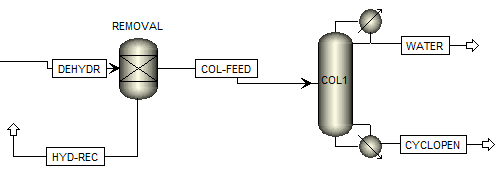
\includegraphics[width=.9\linewidth]{Block_700_-_Καθαρισμός_της_Κυκλοπεντανόνης/2023-01-13_18-02-03_screenshot.png}
\caption{Διάγραμμα ροής του block 700}
\end{figure}

Στο Block 700 λαμβάνει χώρα ο καθαρισμός κυκλόπεντανόνης. Αρχικά, το
ρεύμα εξόδου από τον αντιδραστήρα R-CYCL κατευθύνεται προς έναν
διαχωριστήρα, με σκοπό την αφαίρεση και ανακύκλωση εναπομείναντος
υδρογόνου, το οποίο βρίσκεται στην αέρια φάση. Στη συνέχεια, το ρεύμα
που είναι πλούσιο σε κυκλοπεντανόνη διοχετεύεται σε μια αποστακτική
στήλη, όπου συμβαίνει ο διαχωρισμός για την παραλαβή καθαρής
κυκλοπεντανόνης.

\subsubsection{Σχεδιαστικές Επιλογές}
\label{sec:org26e146c}
Οι δύο βασικές σχεδιαστικές επιλογές του block 700 είναι ο τύπος και η
λειτουργία των δύο στηλών διαχωρισμού.

Για τον διαχωρισμό υδρογόνου χρησιμοποιήθηκε το Component Separator
διότι ο σκοπός είναι να διαχωριστεί το υδρογόνο από το μίγμα
κυκλοπεντανόνης και να χρησιμοποιηθεί με ανακύκλωση στον αντιδραστήρα
R-CYCL. Στην πράξη, καθώς το υδρογόνο είναι ένα αέριο με πολύ χαμηλότερο σημείο βρασμού από ότι όλα τα υπόλοιπα συστατικά, μάλλον μπορεί να ανακτηθεί όλη η ποσότητα του υδρογόνου με ένα flash. Όμως, δεν υπήρχε χρόνος για να δοκιμαστεί αυτό στο Aspen.

Για τον καθαρισμό της κυκλοπεντανόνης χρησιμοποιήθηκε αποστακτική στήλη
DSTWU. Αυτή η αποστακτική στήλη είναι απλή και λειτουργεί με ένα ρεύμα
τροφοδοσίας και δύο προϊόντα απόσταξης. Θα μπορούσε να χρησιμοποιηθεί
κάποια άλλη στήλη όπως η Distl ή η RadFrac, αλλά αυτές πραγματοποιούν
πιο περίπλοκους υπολογισμούς και χρειάζονται περισσότερα δεδομένα.
Επιπλέον, δεν υπάρχει αζεότροπο στο ρεύμα, οπότε δεν χρειάζεται μία πιό αναλυτική επίλυση της στήλης με ένα μοντέλο όπως η στήλη RadFrac.

\subsubsection{Προσομοιώσεις στο Aspen και Υπολογισμοί:}
\label{sec:org4f42304}
Στο Aspen χρησιμοποιήθηκε Component Separator με το θερμοδυναμικό
μοντέλο Peng Robinson με κανόνες ανάμιξης Wong-Sandler (PRWS) για την
πρόβλεψη των θερμοδυναμικών ιδιοτήτων του συστήματος. Για αυτόν λοιπόν
τον separator η πίεση είναι στα 40 bar, ίδιο με την πίεση εξόδου από τον
αντιδραστήρα κυκλοπεντανόνης, και το μίγμα μέσα σε αυτόν είναι διφασικό
(υγρό-ατμός). Μέσω την χρήση του διαχωριστή, το μίγμα που προκύπτει από
τον αντιδραστήρα διαχωρίζεται σε δύο ρεύματα: Το ένα ρεύμα περιέχει
εξολοκλήρου υδρογόνο, το οποίο ανακυκλώνεται στον αντιδραστήρα της
κυκλοπεντανόνης, ενώ το άλλο ρεύμα που περιέχει την κυκλοπεντανόνη, την
φουρφουράλη και το νερό προχωράει στην αποστακτική στήλη για περεταίρω
επεξεργασία.

Πριν να φτάσει το ρεύμα στην αποστακτική στήλη ψύχεται σε εναλλάκτη
θερμότητας σε θερμοκρασία 160 \^{}\{ο\}C και πίεση 20 bar. Το θερμοδυναμικό
μοντέλο για τον εναλλάκτη είναι το ίδιο (PRWS). Στο Aspen ως
εναλλάκτης θερμότητας εφαρμόστηκε Heater. Μετά τη ψύξη του, το ρεύμα
εισέρχεται σε μια αποστακτική στήλη με σκοπό τον διαχωρισμό της
κυκλοπεντανόνης από το νερό.

Αρχικά έγινε χρήση του Azeotrope Finder για την εύρεση αζεότροπων, αλλά
διαπιστώθηκε πως σε πίεση 16 bar δεν υπάρχουν αζεότροπα. Εφόσον η πίεση
του μίγματος είναι 40 bar από τον αντιδραστήρα υδρογόνωσης, επιλέχθηκε
να γίνει απόσταξη σε πίεση 16 bar. Λόγω της έλλειψης αζεότροπων, στο
Aspen έγινε χρήση της απλοποιημένης στήλης DSTWU. Η στήλη περιέχει 55
βαθμίδες απόσταξης και ως προϊόν κορυφής ανακτάται το νερό κατά \(99.9 \%\).
Στο προϊόν κορυφής επιλέγεται η κυκλοπεντανόνη να ανακτάται σε ποσοστό
\(7.7 \%\), εφόσον μικρότερα ποσοστά οδηγούν σε υπερβολικά μεγάλο αριθμό
βαθμίδων και λόγων αναρροής. Η πίεση στον συμπυκνωτή όσο και στον
αναβραστήρα είναι 16 bar, δηλαδή θεωρείται πως δεν υφίσταται πτώση
πίεσης μέσα στην στήλη. Από τους υπολογισμούς του Aspen προκύπτουν τα αποτελέσματα του παρακάτω πίνακα

\begin{table}[htbp]
\caption{Χαρακτηριστικά της αποστακτικής στήλης}
\centering
\begin{tabular}{lr}
Μέγεθος & Τιμή\\
\hline
Ελάχιστος Λόγος Αναρροής & 0.96\\
Πραγματικός Λόγος Αναρροής & 6.61\\
Ελάχιστος Αριθμός Βαθμίδων & 49.39\\
Πραγματικός Αριθμός Βαθμίδων & 55\\
Λόγος αποστάγματος προς τροφοδοσία & 0.813\\
Βαθμίδα τροφοδοσίας & 32\\
\end{tabular}
\end{table}

Ως αποτέλεσμα, το ρεύμα κορυφής έχει μαζική παροχή 1971,2 kg/hr με το
νερό να αποτελεί το \(92.3 \%\) της συνολικής μάζας, και το ρεύμα πυθμένα έχει
μαζική παροχή 1988,7 kg/hr και η κυκλοπεντανόνη αποτελεί το \(98.2 \%\) της
συνολικής μάζας. Τα αποτελέσματα της αποστακτικής στήλης βρίσκονται στον
πίνακα 2. του παραρτήματος.

Στον πίνακα 3. του παραρτήματος απεικονίζονται συνολικά οι μαζικές
παροχές αλλά και οι συστάσεις όλων των ρευμάτων που λαμβάνου χώρα τόσο
για τη παραγωγή όσο και τον καθαρισμό της κυκλοπεντανόνης.

\section{Βιβλιογραφία}
\label{sec:orgc20deb9}
\hypertarget{citeproc_bib_item_1}{(1) Nhien, L. C.; Long, N. V. D.; Lee, M. Novel Hybrid Reactive Distillation with Extraction and Distillation Processes for Furfural Production from an Actual Xylose Solution. \textit{Energies} \textbf{2021}, \textit{14} (4), 1152. \url{https://doi.org/10.3390/en14041152}.}

\hypertarget{citeproc_bib_item_2}{(2) Ershova, O.; Kanervo, J.; Hellsten, S.; Sixta, H. The Role of Xylulose as an Intermediate in Xylose Conversion to Furfural: Insights via Experiments and Kinetic Modelling. \textit{Rsc advances} \textbf{2015}, \textit{5} (82), 66727–66737. \url{https://doi.org/10.1039/C5RA10855A}.}

\hypertarget{citeproc_bib_item_3}{(3) Papaioannou, M.; Kleijwegt, R. J. T.; van der Schaaf, J.; Neira d’Angelo, M. F. Furfural Production by Continuous Reactive Extraction in a Millireactor under the Taylor Flow Regime. \textit{Industrial \& engineering chemistry research} \textbf{2019}, \textit{58} (35), 16106–16115. \url{https://doi.org/10.1021/acs.iecr.9b00604}.}

\hypertarget{citeproc_bib_item_4}{(4) Carrasco, F. Production of Furfural by Dilute-Acid Hydrolysis of Wood: Methods For Calculating Furfural Yield. \textit{Wood and fiber science} \textbf{1993}, 91–102.}

\hypertarget{citeproc_bib_item_5}{(5) Yu, Z.; Li, Y.; Yao, Y.; Wang, Y.; Liu, Y.-Y.; Sun, Z.; Shi, C.; Wang, W.; Wang, A. Highly Selective Hydrogenative Ring-Rearrangement of Furfural to Cyclopentanone over a Bifunctional Ni3P/\$\gamma\$-Al2O3 Catalyst. \textit{Molecular catalysis} \textbf{2022}, \textit{522}, 112239. \url{https://doi.org/10.1016/j.mcat.2022.112239}.}

\section{Παράρτημα E}
\label{sec:org33d5669}
\begin{figure}[htbp]
\centering
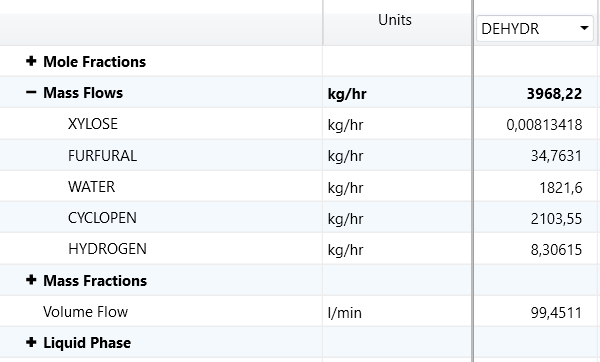
\includegraphics[width=.9\linewidth]{Παράρτημα/2023-01-13_18-10-03_screenshot.png}
\caption{Ρεύμα εξόδου από τον αντιδραστήρα R-CYCL για την παραγωγή της κυκλοπεντανόνης}
\end{figure}

\begin{figure}[htbp]
\centering
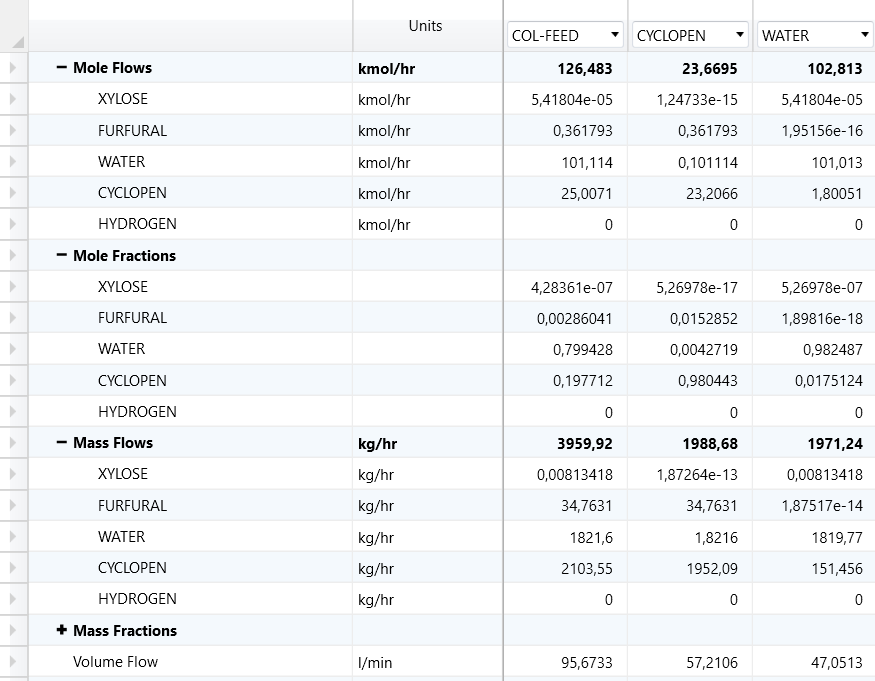
\includegraphics[width=.9\linewidth]{Παράρτημα/2023-01-13_18-10-10_screenshot.png}
\caption{Αποτελέσματα Αποστακτικής Στήλης}
\end{figure}

\begin{figure}[htbp]
\centering
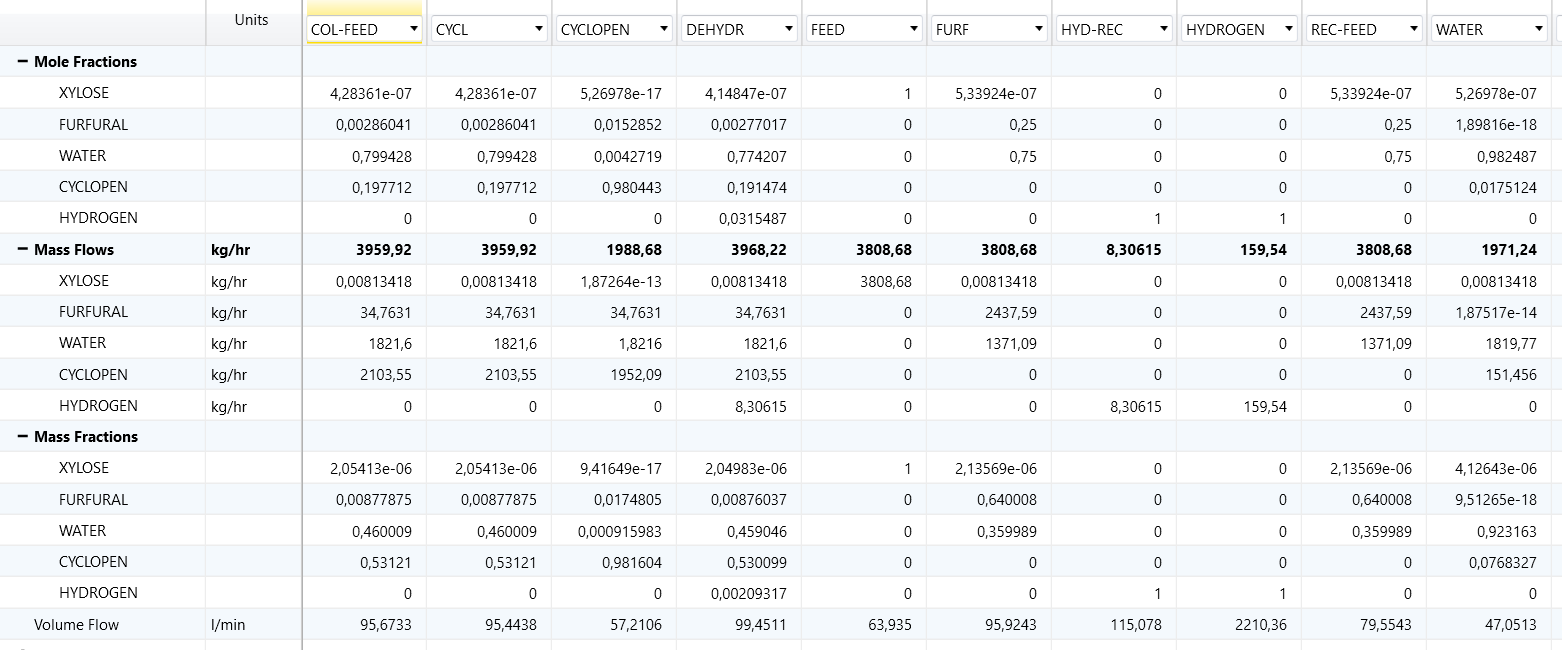
\includegraphics[width=.9\linewidth]{Παράρτημα/2023-01-13_18-10-19_screenshot.png}
\caption{Αποτελέσματα συνολικής διεργασίας για την κυκλοπεντανόνη}
\end{figure}
\end{document}